\documentclass[10pt]{article}

% amsmath package, useful for mathematical formulas
\usepackage{amsmath}
% amssymb package, useful for mathematical symbols
\usepackage{amssymb}

% graphicx package, useful for including eps and pdf graphics
% include graphics with the command \includegraphics
\usepackage{graphicx}

% cite package, to clean up citations in the main text. Do not remove.
\usepackage{cite}

\usepackage{color} 

% Use doublespacing - comment out for single spacing
\usepackage{setspace} 
\doublespacing

% Text layout
\topmargin 0.0cm
\oddsidemargin 0.5cm
\evensidemargin 0.5cm
\textwidth 16cm 
\textheight 21cm

% Bold the 'Figure #' in the caption and separate it with a period
% Captions will be left justified
\usepackage[labelfont=bf,labelsep=period,justification=raggedright]{caption}

% Use the PLoS provided bibtex style
\bibliographystyle{plos2009}

% Remove brackets from numbering in List of References
\makeatletter
\renewcommand{\@biblabel}[1]{\quad#1.}
\makeatother


% Leave date blank
\date{}

\pagestyle{myheadings}
%% ** EDIT HERE **


%% ** EDIT HERE **
%% PLEASE INCLUDE ALL MACROS BELOW

% figure files reside in the figures/ directory
\graphicspath{
{figures/}
}

%% END MACROS SECTION

\begin{document}

% Title must be 150 characters or less
\begin{flushleft}
{\Large
\textbf{Spatially explicit model of the lymphocyte diaspora in influenza-infected lung quantifies constraints of chemokine directed migration}
}
% Insert Author names, affiliations and corresponding author email.
\\
Drew Levin$^{1,\ast}$, 
Stephanie Forrest$^{1}$, 
Soumya Banerjee$^{1}$
Candice Clay$^{2}$, 
Melanie Moses$^{1}$, 
Frederick Koster$^{2}$, 
\\
\bf{1} Department of Computer Science, University of New Mexico, Albuquerque, NM, USA
\\
\bf{2} Lovelace Respiratory Research Institute, Albuquerque, NM, USA
\\
$\ast$ E-mail: Corresponding drew@cs.unm.edu
\end{flushleft}



% Please keep the abstract between 250 and 300 words
\section*{Abstract}

During the primary immune response, clearance of influenza in the lung requires the homing of activated CD8 T cells during the lymphocyte diaspora from regional lymph nodes to small infected foci representing a tiny fraction of the total lung.  T-cell navigation through the complex branching bronchial vascular network is enabled by local cytokine and chemokine production from infected epithelial cells.  Avian H5N1, seasonal H1N1, and 2009 pandemic influenza strains were used separately to induce chemokine production \textit{in vitro}.  Of the eight chemokines tested only CXCL10 (IP-10) and CCL5 (RANTES) were secreted in tissue  (results only) with IP-10 always dominating the affected T-cell migration direction.  A delayed differential equation model was fit to the empirical data, revealing per cell chemokine production rates for each strain.  These values were coupled with known biological constants to calibrate a spatially explicit agent-based model to explore the effects of inter-strain variation of chemokine production on T-cell recruitment.  In the model immune response is unable to clear the infection of pandemic H1N1 influenza due to the high rate of viral production and plaque size expansion.  The spatial nature of the model reveals unique challenges to T-cell recruitment and motility not visible in spatially homogeneous ODE models.  Expanding plaque sizes isolate infected cells, causing T-cell discovery and subsequent clearance of the infection to become less effective over time.  

% Please keep the Author Summary between 150 and 200 words
% Use first person. PLoS ONE authors please skip this step. 
% Author Summary not valid for PLoS ONE submissions.   
\section*{Author Summary}


\section*{Introduction}

The adaptive immune response induced during acute influenza A infection is a complex web of defense mechanisms that controls all but the most virulent strains.  Understanding its components and their interactions are relevant to improving vaccines and strategies to control immunopathology. Elegant studies in the mouse model have described the induction and effector phases of the adaptive immune response, including functional capabilities of the innate interferon-directed response, macrophages, specific antibody, and cytotoxic effector lymphocytes \cite{Sallusto2000, Joo2008, Mackay2008}.   CD8+ T cells are necessary for the resolution of pneumonia and complete clearance of mouse-adapted influenza strains \cite{Sallusto2000, Joo2008, Mackay2008, Miao2010}, but gaps remain in our understanding of the behavior of activated T cells in infected tissue.

The generally held view of the sequence of CD8+ T cell events during a primary immune response to influenza in the lung involves the following steps: dendritic cells bearing specific antigen migrate from the lung to the draining lymph node where naive T and B cell precursors are activated in specialized architecture \cite{Saenz2010, Beltman2007, Handel2008, Zheng2008, Ingulli2009, Allan1990}.  T cells proliferate in the lymph node and are released into the bloodstream, appearing simultaneously in the lung, spleen and other organs 4-5 days post-infection, a whole-body distribution known as the lymphocyte diaspora \cite{Thelen2008}.  In the lung, extravasation from capillaries is signaled by inflammatory cytokine-mediated integrin-activation on endothelial cells.  Once in the tissue, T cells follow a chemokine gradient to the infected epithelial cells secreting the chemokine.

Mathematical models have used detailed mouse data to characterize the evolution of the immune response and predict its impact on viral kinetics \cite{Thomas-Vaslin2008, Beauchemin2008, Smith2010, Thakar2010, Burrowes2004}.  Such whole-response modeling has considerable potential to inform strategies of vaccination and therapy, thus avoiding subsequent expensive animal and human trials.  Models using ordinary differential equations to predict temporal events, however, do not account for spatial constraints, and must make assumptions about the efficiency of the spread and interaction of populations. 

Here we focus on the time and physical constraints of the lymphocyte diaspora using an agent-based model (ABM).  To develop a model with tractable simulations, some key components of host defense are not incorporated explicitly and the model therefore does not aim to predict the true outcome for each strain examined.   We ask how do very small foci of infected tissue attract limited numbers of activated CD8 T cells after release into the systemic vascular system.  The circulating blood supply services non-infected tissue orders of magnitude larger than the target infected tissue, necessitating an efficient mechanism to focus cell migration.   A host of cytokines and chemokines secreted by infected cells are critical in directing immune cells to sites of infection \cite{Miao2010, Zhao2000, LiJeon2002}.  While each chemokine has been studied in detail for receptor specificity and function in knockout models, the details of chemokine function and efficiency have not been examined in a virus-infected whole animal model.  

To characterize the local chemokine-secretion environment in which T cells migrate, we used data on viral secretion and chemokine secretion patterns from human epithelial cells infected in vitro by three different influenza virus strains of avian, seasonal and pandemic origins \cite{Mitchell2011}.   We selected in vitro chemokine data as a tissue environment surrogate, because it may be more accurate than published chemokine levels in mouse blood and bronchial alveolar fluid, and it allowed us to represent sustained chemokine gradients within the model lung.  Extensive literature on mouse model data of infections with mouse-adapted strains PR8 and HK-31 were used to populate the ABM model with activated CD8+ T cells. [REF]

The standard hypothesis would posit that in this model the marked strain-specific differences in replication efficiency and tissue spread previously reported \cite{Mitchell2011} would largely determine the outcome of infection as eradication or lack of control.  While we found this to be true, we observed three interesting characteristics of chemokine-directed migration not revealed from experimental data.  First, of the only two chemokines stimulated by all three strains, the influence of IP-10 consistently dominated the effect of RANTES, regardless of strain.  Second, each chemokine exhibited a clear threshold to direct migration, with lesser impact at increasing concentrations above the threshold.  Finally, when the target (infection focus) was large, T cell search became inefficient due to the disappearance of the chemokine gradient, possibly contributing to the loss of control of the pandemic strain.  

% You may title this section "Methods" or "Models". 
% "Models" is not a valid title for PLoS ONE authors. However, PLoS ONE
% authors may use "Analysis" 
\section*{Models}


\subsection*{Computational Modeling}

\begin{figure}[ht!]
\begin{center}
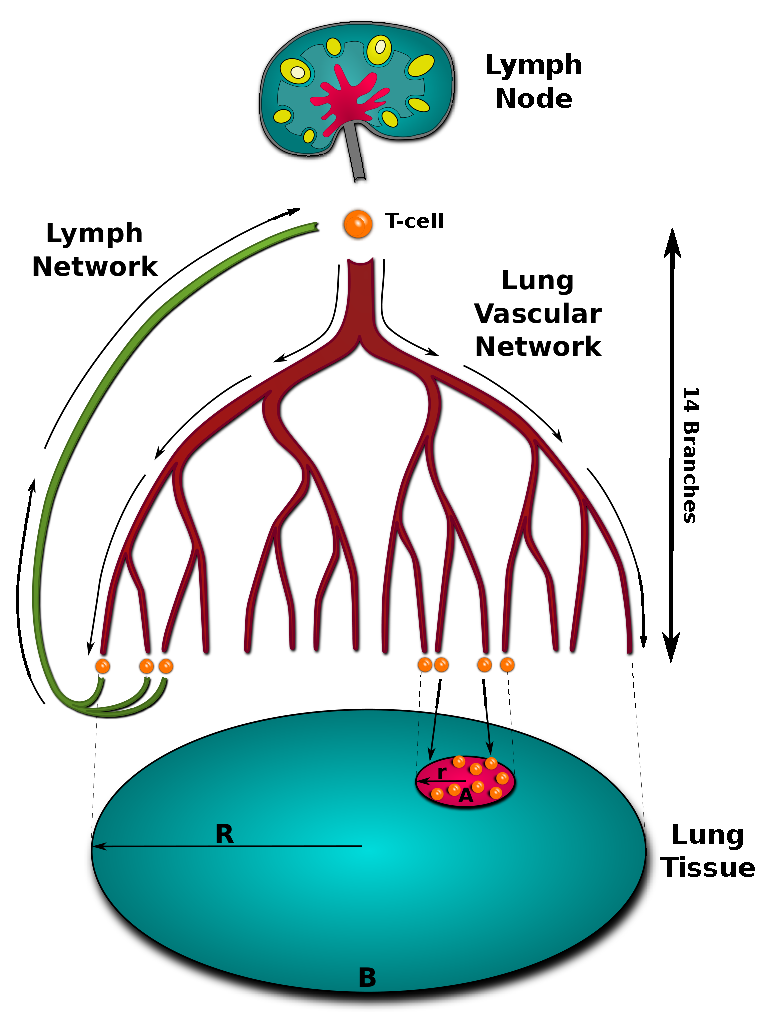
\includegraphics[width=0.5\textwidth]{SystemChart}
\end{center}
\caption{A simplified model of T cell search.  Activated T cells originate in the lymph node and enter the bloodstream after which they randomly navigate through the 14 layers of the branching bronchial network.  Upon reaching a capillary, T cells will exit into the tissue in the presence of a cytokine signal.  T cells that do not sense a signal will continue to recirculate either through the lymph network or through the pulmonary vein back to the top of the network.}
\label{fig:systemchart}
\end{figure}

Computational modeling was conducted using CyCells \cite{Warrender2006}, a modeling platform for two- or three-dimensional agent-based simulations of the immune response. A simplified model of T-cell activation and recirculation was implemented in CyCells (Fig.~\ref{fig:modelchart}) and simulations were conducted to measure efficiency of infection clearance under different environmental conditions. To model a growing infection, the lung was represented as a two dimensional sheet of healthy epithelial cells. Vasculature was represented as a binary tree with fourteen branches originating at a single lymph node. Activated T cells descend through the vascular tree until cytokine signal is detected, at which point they exit the vasculature and follow the chemotactic gradient to the site of infection. T cells that do not encounter cytokine recirculate to the lymph node. At the site of infection when a T cell encounters an infected epithelial cell it induces apoptosis.

The simulation begins when a single cell in the center of the tissue is infected. After the eclipse phase (incubation), the infected cell begins secreting virus and chemokine. Virus diffuses locally, infecting nearby cells, and continuing the cycle. Chemokine also diffuses from secreting cells, creating a ball of stimulation around the infected region. After a delay to simulate lymph node stimulation and T cell proliferation, activated T cells begin exiting the lymph node and circulating through the vasculature to the tissue. Because T  cells cannot choose their path through the branching network, we assume they arrive in tissue at random locations. 


\subsection*{Model Definition}

\begin{figure}[ht!]
\begin{center}
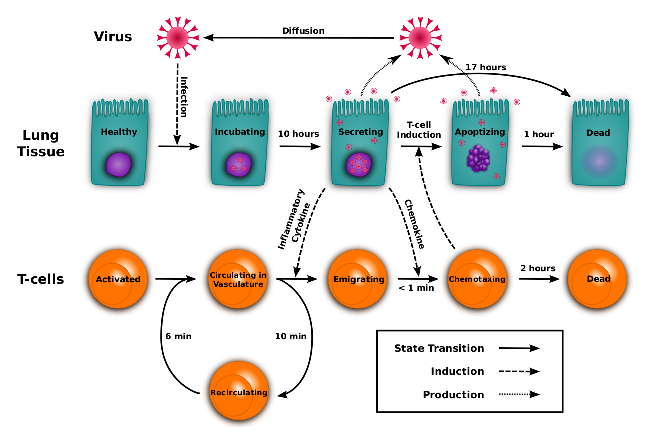
\includegraphics[width=\textwidth]{ModelChart}
\end{center}
\caption{A visual representation of the model.  Healthy epithelial cells infected by virus begin secreting virus after an incubation delay.  T cells are activated in the lymph node and traverse the bronchial vascular network to the site of infection where they are recruited by inflammatory cytokine.  Chemotaxing T cells climb the chemokine gradient and induce apoptosis in infected cells.  Solid arrows represent the transition of a cell from one behavioral state to another.  Dashed arrows display the mechanism used to induce a transition.  Dotted arrows show the production of new virus.}
\label{fig:modelchart}
\end{figure}

Epithelial cells are stationary and can be in one of five different states: \emph{healthy}, \emph{virus-incubating}, \emph{virus-expressing}, \emph{apoptotic}, and \emph{dead}. \emph{Healthy} cells remain unchanged unless infected by virus. Once infected, the cell transitions from {incubating} to \emph{expressing}. \emph{Expressing} cells secrete virus and chemokine for 17 hours and then die. \emph{Expressing} cells become \emph{apoptotic} if they encounter activated T-cells. Apoptoic cells continue to secrete virus until they die one hour after their transition. \emph{Dead} cells remain inert and do not regenerate over the course of an infection.

T-cells have three states: \emph{searching}, \emph{recirculating}, and \emph{chemotaxing}. \emph{Searching} T-Cells begin emerging from the lymph node at five days post infection. These T-Cells arrive at a random location on the lung's surface, perform a random walk in the tissue for 10 minutes and transition to \emph{circulating} in the absence of chemokine. \emph{Circulating} cells spend six minutes recirculating to the lymph node, transition to \emph{searching} and are reintroduced to a new random location in the lung. When a \emph{searching} T-Cell encounters chemokine, it converts to \emph{chemotaxing} and begins climbing the chemotactic gradient to the source of infection. \emph{Chemotaxing} T-Cells move continuously up the gradient, inducing apoptosis if they encounter \emph{expressing} epithelial cells. \emph{Chemotaxing} decay exponentially with an average lifespan of two hours. 

The model contains two kinds of particles: virus and chemokine. Both are produced at constant rates by \emph{expressing} epithelial cells.  Virus diffuses through the lung tissue, infecting healthy cells probabilistically according to the local virus concentration. Chemokine diffuses across the tissue but has no
direct effect beyond activating T-Cells. Both particle types decay exponentially.

Parameters that are consistent between every model are shown in Table \ref{table:parameters}.  Strain-specific values are shown in Table \ref{table:strains}.

\begin{table}
\begin{center}
\begin{tabular}{ | c | c | c | }
  \hline                        
  Paramter & Value & Source \\
  \hline
  Viral Diffusion & .0318 & \cite{Beauchemin2006} \\
  Viral Decay &  $1/day$ & Phenomenological \\
  Chemokine Diffusion & $.318 \mu m^2/s$ & \cite{Beauchemin2006} \\
  Chemokine Decay &  $3.8508$e-4$/s$ & 30m half-life \\
  Infection Sensitivity &  $2 h/virion$ & Phenomenological \\
  Incubation Time &  $10 h$ & \cite{Mitchell2011} \\
  Expression Time &  $16.7 h$ & \cite{Mitchell2011} \\
  Apoptosis Time & $1 h$ & Phenomenological \\
  T-Cell Production Rate & $777/h$ & \cite{Miao2010} \\ 
  Circulation Time & $6 m$ & \cite{Banerjee2010b} \\
  Search Time & $10 m$ & \cite{Banerjee2010b} \\
  T-Cell Speed (Search) & $30 \mu m/s$ & \cite{Miller2003} \\
  T-Cell Speed (Activated) & $3 \mu m/s$ & \cite{Miller2003} \\
  T-Cell Sensitivity & $1 ng/mL$ & \cite{Gao2003} \\
  T-Cell Expected Kill Rate & $10 m$ & [REF] \\
  Cell Radius & $25 \mu m$ & Phenomenological \\
  T-Cell Age (at FOI) & $2 h$ & [REF] \\
  T-Cell Age (Other) & $3 d$ & [REF] \\
  T-Cell Ramp Up Time & $5 d$ & \cite{Banerjee2011} \\
  IgM Strength & Viral decay of $3/day$ & Phenomenological \\
  \hline  
\end{tabular}
\caption{Generic model parameters}
\label{table:parameters}
\end{center}
\end{table}


\begin{table}
\begin{center}
\begin{tabular}{ | r | c | c | }
  \hline                        
  Paramter & Value & Source \\
  \hline
  IP-10 Production Rate &  & ODE Fits \\
  Avian H5N1 & 2.0e-4 pg/s$\cdot$cell & \\
  Seasonal H1N1 & 1.8e-4 pg/s$\cdot$cell& \\
  Pandemic H1N1 & 8.7e-5 pg/s$\cdot$cell& \\
  \hline
  RANTES Production Rate & & ODE Fits \\
  Avian H5N1 & 1.3e-5 pg/s$\cdot$cell& \\
  Seasonal H1N1 & 8.9e-7pg/s$\cdot$cell& \\
  Pandemic H1N1 & 4.4e-6 pg/s$\cdot$cell& \\
  \hline
  Virus Production Rate &  & \cite{Mitchell2011} \\
  Avian H5N1 & 5.4e-5 PFU/s$\cdot$cell& \\
  Seasonal H1N1 & 3.8e-4 PFU/s$\cdot$cell& \\
  Pandemic H1N1 & 5.1e-3 PFU/s$\cdot$cell& \\  
  \hline  
\end{tabular}
\caption{Strain specific model parameters}
\label{table:strains}
\end{center}
\end{table}

\section*{Materials}

Chemokine secretion:  Epithelial cell culture and supernatant collection was performed as described \cite{Mitchell2011}.  Briefly, undifferentiated human tracheal epithelial cells (University of Miami) were cultured for 4 weeks to achieve fully differentiated confluent monolayers on collagen-coated transwell inserts, or commercial differentiated human bronchial epithelial cells (EpiAirway Tissue, MatTek Corp., Ashland, MA) used immediately upon receipt, were infected at an MOI of 0.01 with either seasonal H1N1 virus A/New Caledonia/20/99 (sH1N1), the 2009 H1N1 pandemic strain A/California/04/09 (pH1N1), or avian H5N1 virus A/Hong Kong/483/97 (aH5N1) derived from a fatal human infection.  Apical fluid for viral secretion, and basal media for chemokine secretion collected before treatment of the monolayer with protease, was collected from previously undisturbed triplicate or quadruplicate wells at 0, 6, 10, 12, 16, 20, 24, 30, 36, 42, 48, and 72 hours after infection, and stored at -80C until assay.  Quantitative viral culture was performed by standard plaque assay.  Quantitative chemokine levels were performed in 30 µl aliquots for a panel of 17 chemokines and cytokines (Luminex Assay®, Luminex Corp.) and reported as ng/mL basal media sampled from a total volume of 4 mL.

% Results and Discussion can be combined.
\section*{Results}

\subsection*{Chemokine production}

Chemokine data were collected from epithelial monolayers infected with influenza strains, as described in \cite{Mitchell2011} (Fig.~\ref{fig:data}).  IP-10 concentration increases were observed by 8h p.i., and RANTES by 16h p.i..  To estimate per-cell production rates, we extended the ODE model of Ref. \cite{Mitchell2011} to represent chemokine production from infected cells.  Model fits, shown in Table \ref{table:strains}, were generated for three influenza strains (Fig.~\ref{fig:data}) using a genetic algorithm \cite{Mitchell2011}.  These expression rates are similar across different strains with the exception of significantly higher RANTES production in aH5N1.  There is no discernible correlation between viral production and induced chemokine production across the three strains.

\begin{figure}[ht!]
\begin{center}
 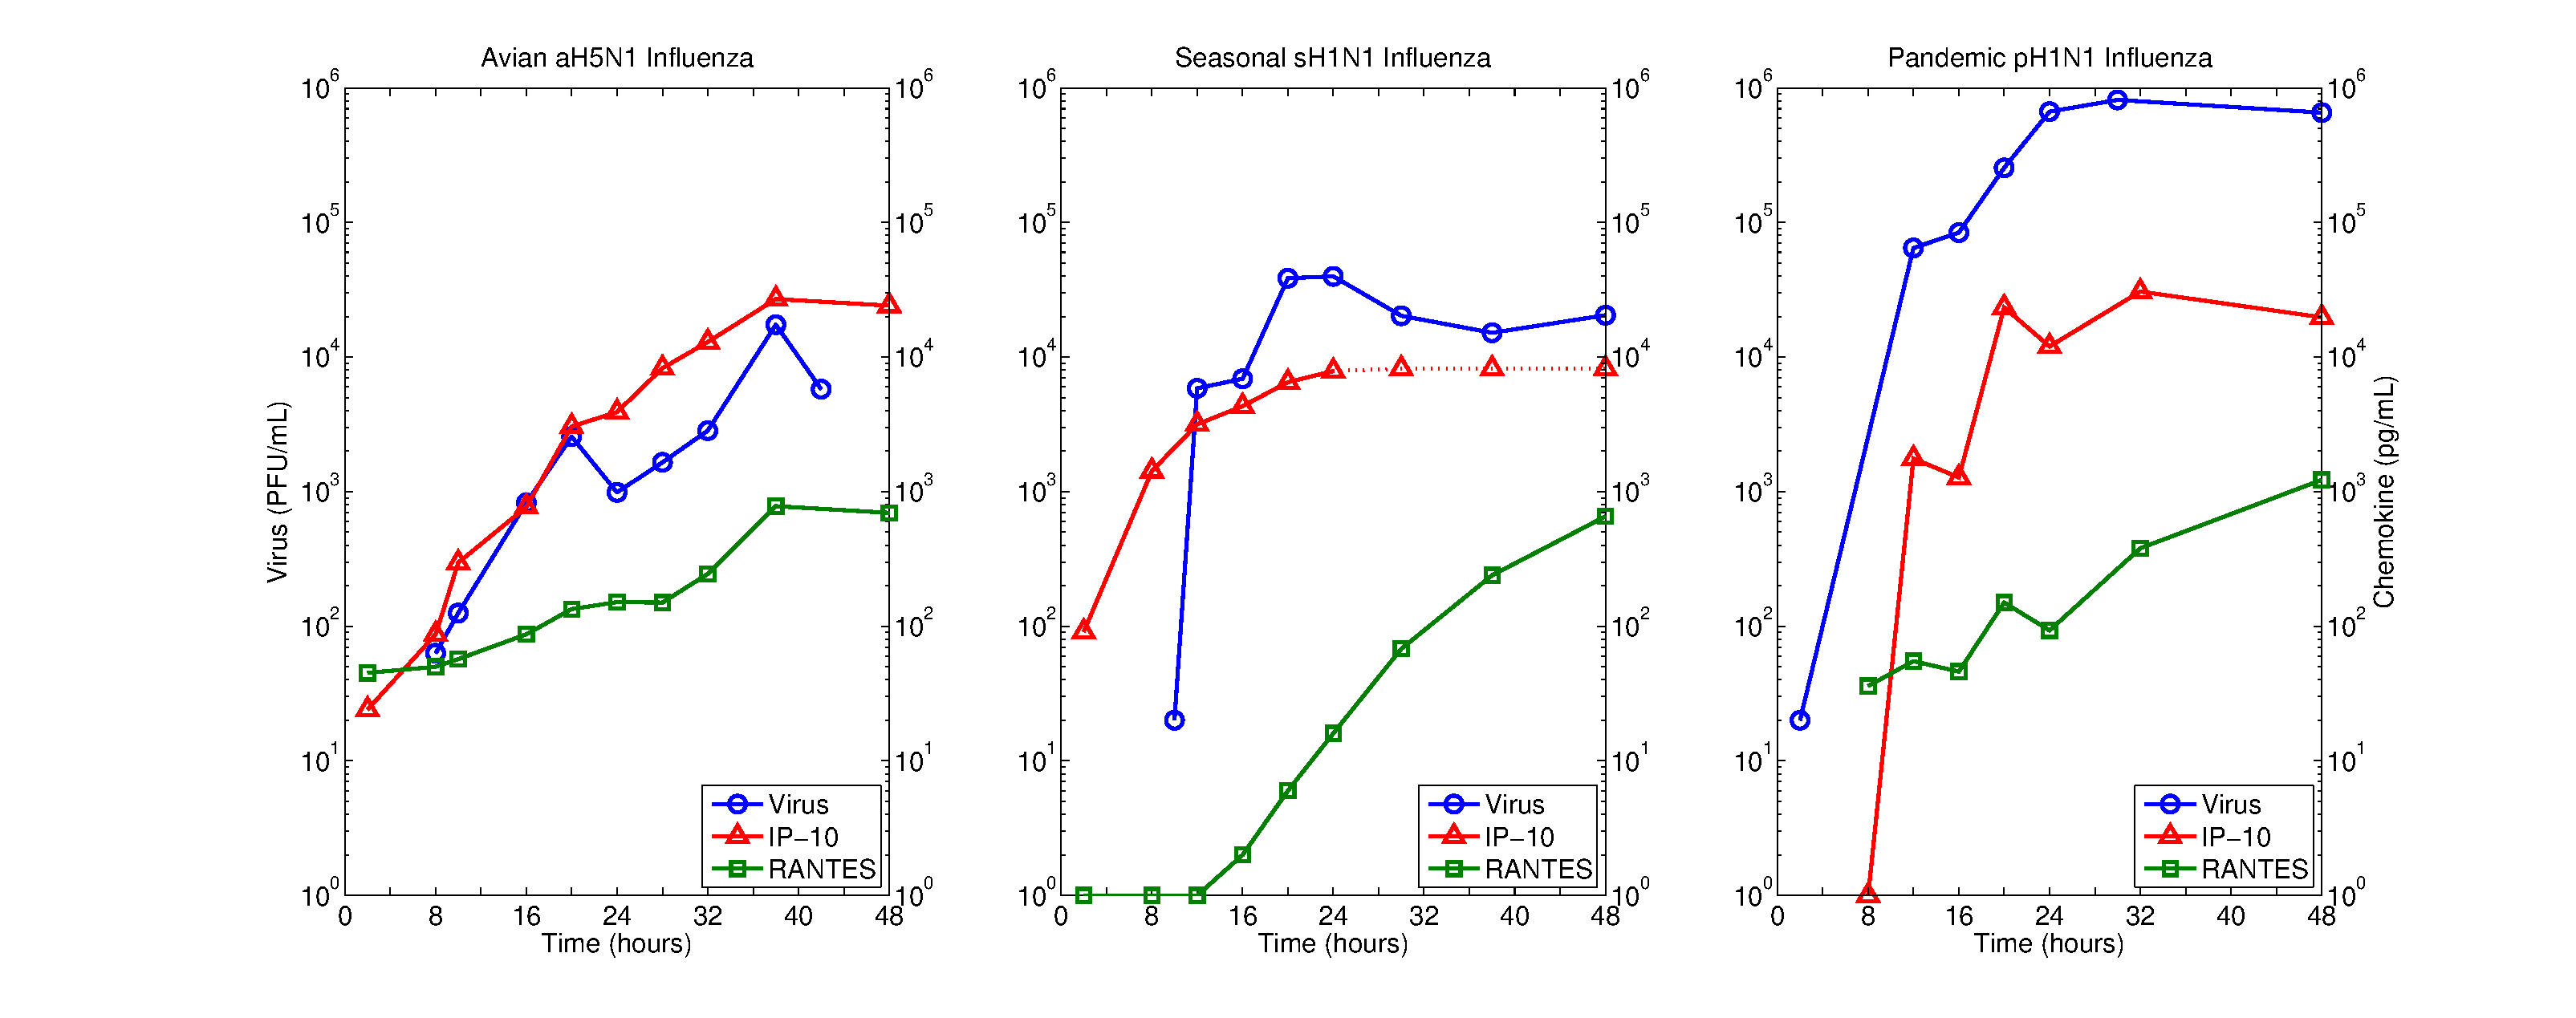
\includegraphics[width=\textwidth]{data}
 \end{center}
\caption{Empirical data of viral and cytokine titer for three strains of influenza: Avian H5N1 (A), Seasonal sH1N1 (B), and Pandemic pH1N1 (C).  For each strain, the viral load (blue circle) is shown in PFU/mL and the chemokines IP-10 (red triangle) and RANTES (green square) are shown in ng/mL.  sH1N1 IP-10 registered three values not included in model fitting above the measurement threshold of 8,500 $pg/mL$ (dotted line).} 
 \label{fig:data}
\end{figure}


\subsection*{T-cell sensitivity to chemokine}

T-Cells exit a capillary when they sense inflammatory cytokine and follow the chemokine gradient.  The model uses chemokine gradient as a surrogate for the inflammatory response.  Figure \ref{fig:cycells} shows chemokine concentrated around virus secreting cells.  T-cell sensitivity determines how much aggregate chemokine signal is required to detect the gradient.

To test for the minimum concentration of cytokine/chemokine signal required to recruit T-Cells from capillary, we simulated sensitivity levels ranging over seven orders of magnitude. We find a threshold (Fig.~\ref{fig:sensitivity}) between the concentrations of 1 $\mu g/ml$ and 100 $ng/ml$ (100 $ng/ml$ and 10 $ng/ml$ in aH5N1), below which there is no discernible effect on infection kinetics.  Because multiple T-cells in the same area do not increase apoptosis, we hypothesize that above a critical threshold no additional benefit is conferred by increasing T cell presence.  We use the sensitivity of 10 $ng/mL$ for each run, which corresponds to a $1 nM$ concentration assuming a chemokine molecular weight of 10 $kDa$ \cite{Gao2003}.

\begin{figure}[ht!]
\begin{center}
 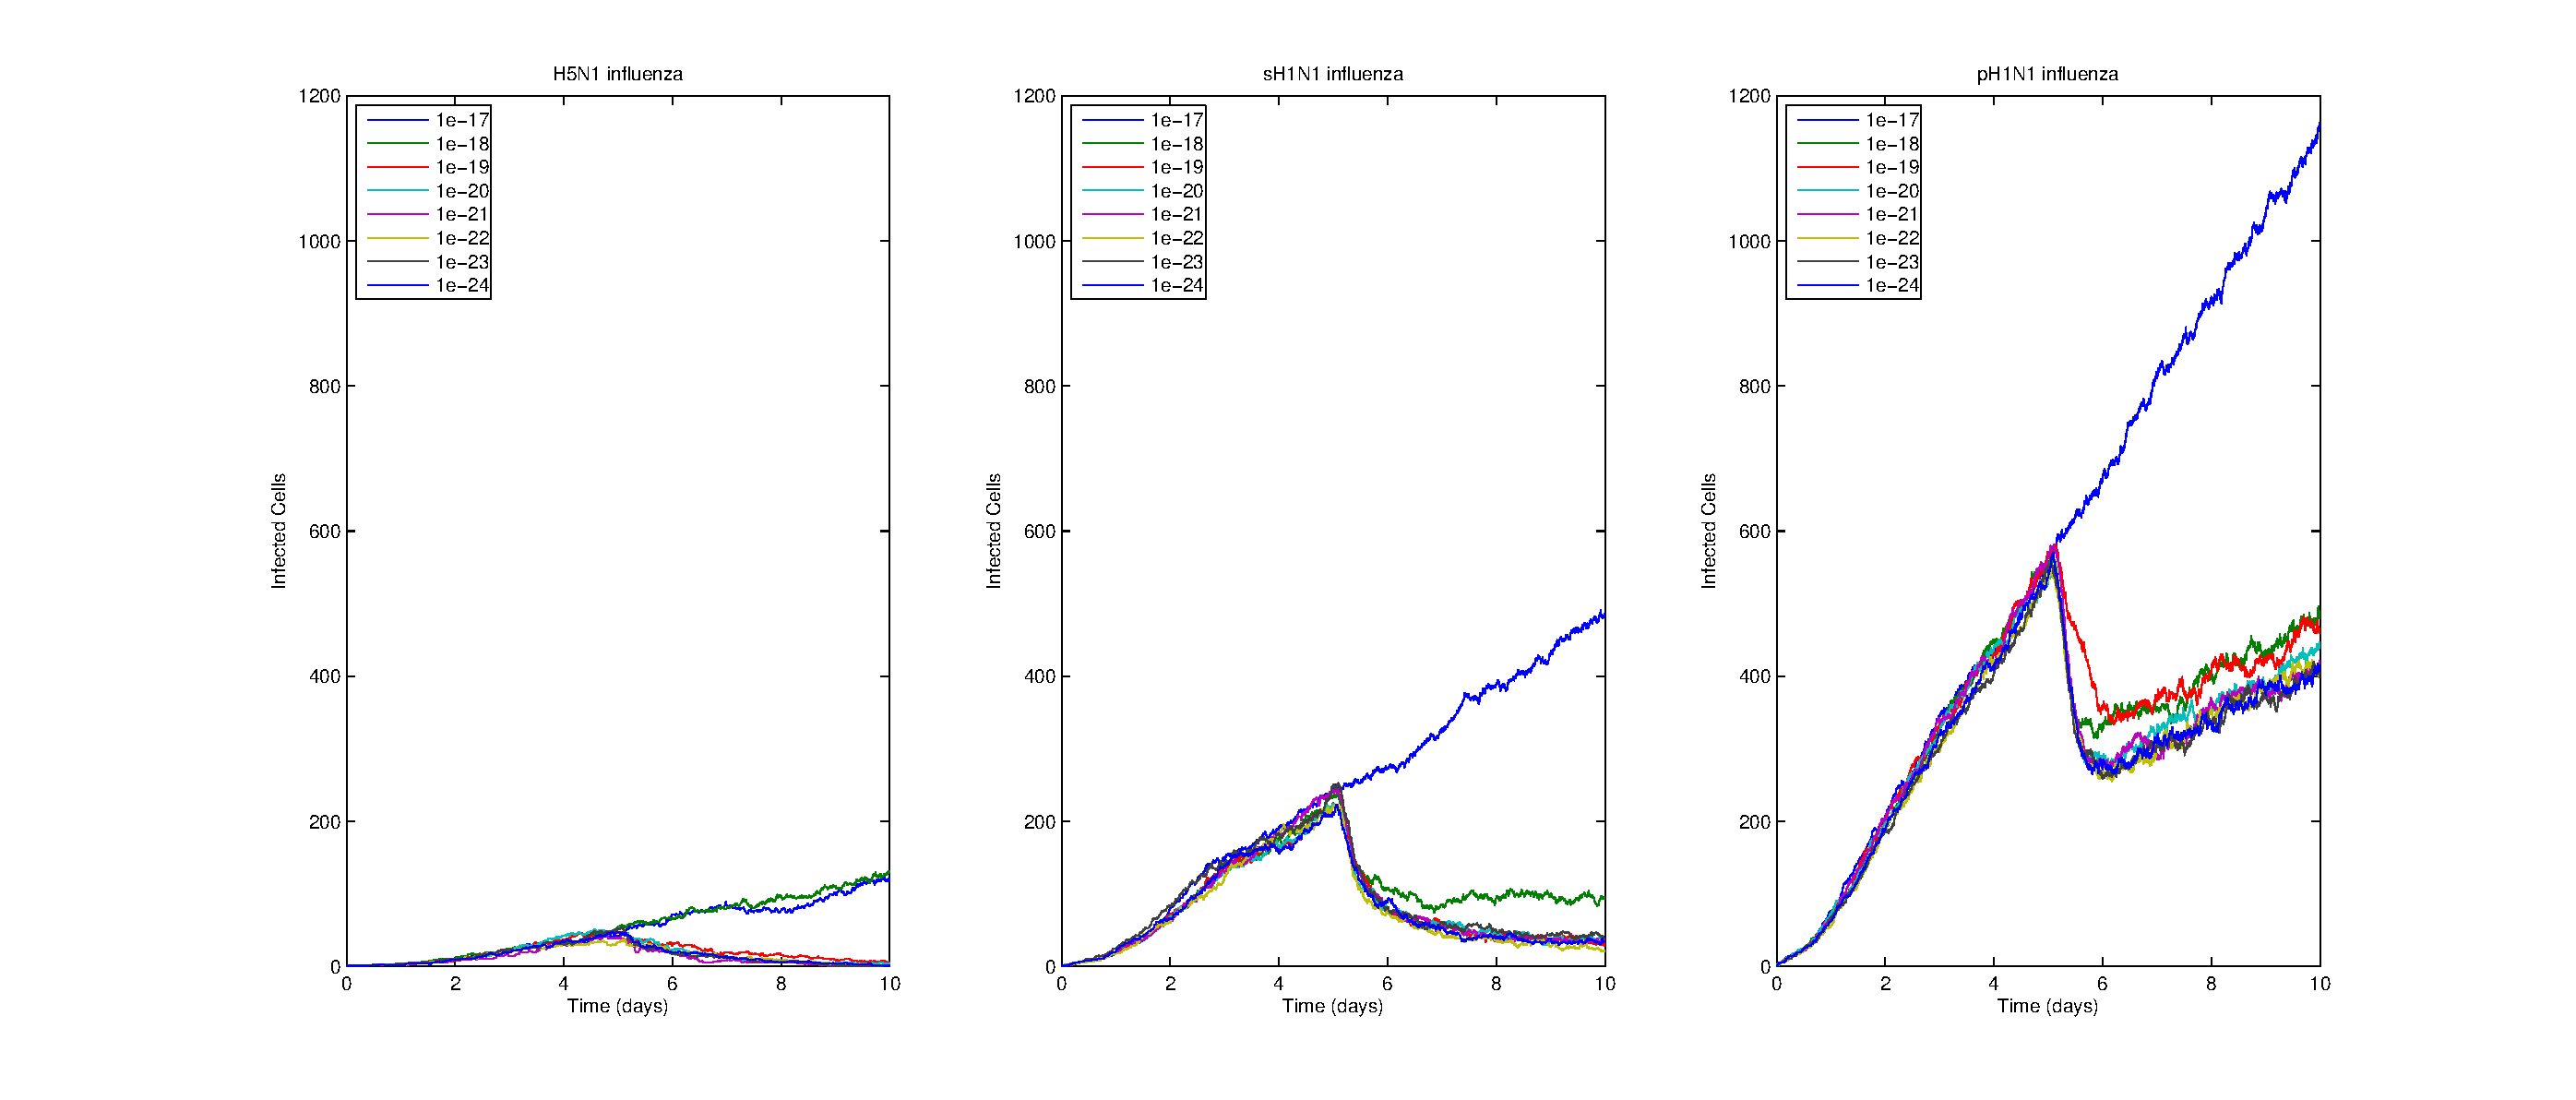
\includegraphics[width=\textwidth]{sensitivity}
 \end{center}
\caption{Varying T-cell sensitivity to chemokine in the model: H5N1 model results use RANTES  only, and sH1N1 and pH1N1 use both IP-10 and RANTES. Total number of infected, expressing and apoptotic cells are plotted for each infection.  The sensitivity value specifies the minimum level of chemokine concentration required for T-cells to detect it. } 
 \label{fig:sensitivity}
\end{figure}


\subsection*{Spatial effects}

Spatial effects of viral and chemokine diffusion play an important role in both the spreading and clearing infections.  Free virus particles diffuse from virus secreting cells and infect healthy cells.  Chemokine produced by infected cells attracts T-cells to the infected cells.  Although virus is produced at a higher rate than chemokine, the larger particle diffuses much more slowly.  Chemokine diffusion decays more quickly.  These countervaling effects result in similar spatial profiles for the two particle types (Fig.~\ref{fig:cycells}).

Up to day 4 the plaque is dominated by active (incubating and secreting) cells, and dead cells are rare. Over time, cells in the plaque's interior die, and active cells are a decreasing proportion of the plaque. T-cells arrive at day 5 and begin killing the virus-secreting cells. By day 6 many expressing cells have been eliminated and the plaque is dominated by dead cells.  In H5N1, the plaque is dense, allowing T-cells to find secreting cells easily and infection is eliminated.  However, in both H1N1 simulations secreting cells were not eliminated.  Expressing cells accounted for at most 10\% of the active cell population and less than 1\% of the total plaque at 6 days p.i..  T cells still accumulate, but they arrive more slowly than the plaque is growing, leading to lower average T cell killing rate.  Further, the regions of concentrated chemokine lag behind the cell and virus spatial layout.  It takes time for newly secreting cells to produce chemokine while pockets of high chemokine density are slow to decay.  Thus, T-cells can lag behind cellular changes in the plaque.  Taken together, the delayed response and low proportion of virus secreting cells prevent T-cells from completely clearing the infection.

The immune response fails to clear sH1N1 completely and is unable to contain pH1N1 (Fig. \ref{fig:sensitivity}).  T-cells are unable to kill cells that have not yet presented antigen.  At day 5.5, the ratio of secreting cells to the total plaque size is high (Fig.~\ref{fig:cycells}). By day 7, this ratio is approximately 1:100 for both the pH1N1 and sH1N1 strains.  The high replication rate of pH1N1 enhances this effect (Fig.~\ref{fig:plaquesize}C) and the T-cells can control (but not eliminate) the sH1N1 infection.

A cell infected with pH1N1 produces new virus at the rate of 5.08e-3 PFU/s \cite{Mitchell2011}.  That is, a new viral particle is produced approximately every 200 seconds.  Assuming that secretion continues for one hour after apoptosis is initiated, the best a T-Cell can do is to limit production to 18 new viral particles.  T-Cells alone cannot contain the pH1N1 infection.  In contrast, a sH1N1 virus-secreting cell produces a new virus particle every 2,643 seconds, allowing T-cells to limit a single infected cell to 1.3 viral particles in the one-hour window.  Avian H5N1 virus-secreting cells produce only 0.2 viral particles in the interval after T-cell detection. 

\begin{figure}[ht!]
\begin{center}
 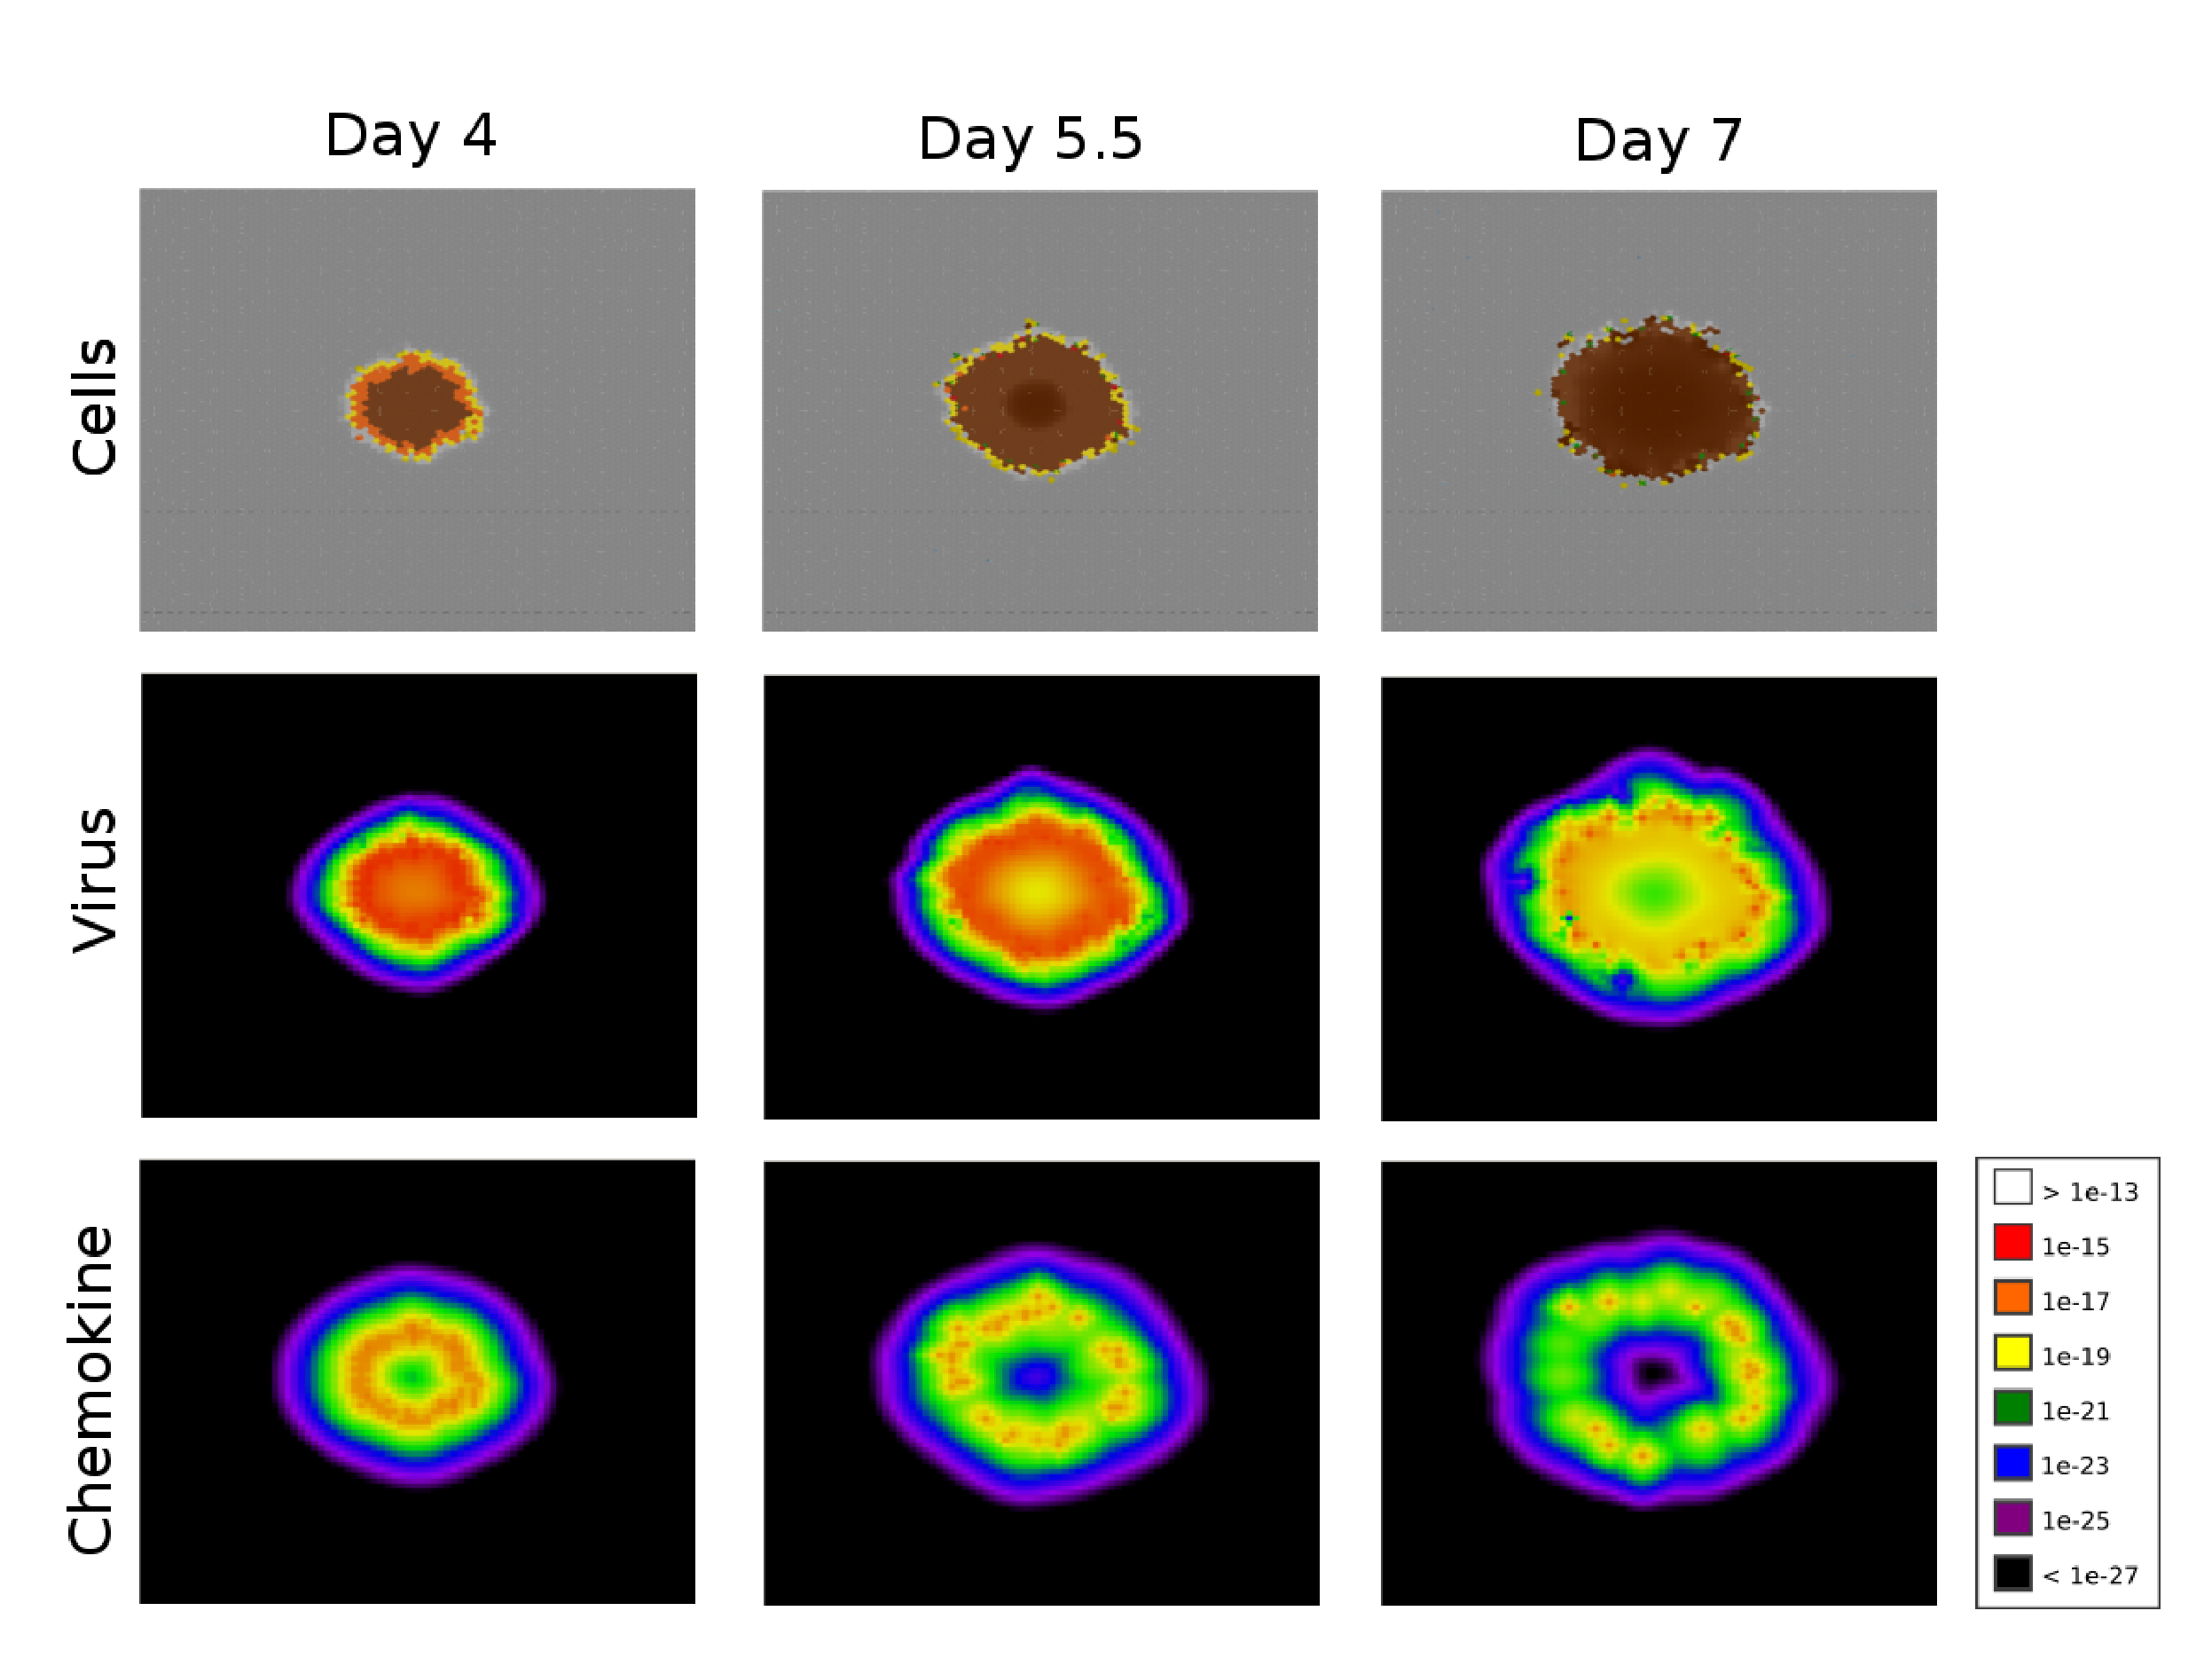
\includegraphics[width=\textwidth]{cycells}
 \end{center}
\caption{A sH1N1 infection in CyCells. Screenshots taken at Day 4, Day 5.5, and Day 7.  The top row shows the spreading focus of infection  through the color coding of individual cells:  healthy cells in uninfected tissue (gray),  virus-incubating cells (yellow), virus-secreting cells (orange), apoptotic cells (red), dead cells (brown), and T-cells introduced at day 5 (green).  Free virus and chemokine particles are represented by compartmentalized concentrations of mols/mL and ng/mL (see the legend in the bottom right).} 
 \label{fig:cycells}
\end{figure}


\begin{figure}[ht!]
\begin{center}
 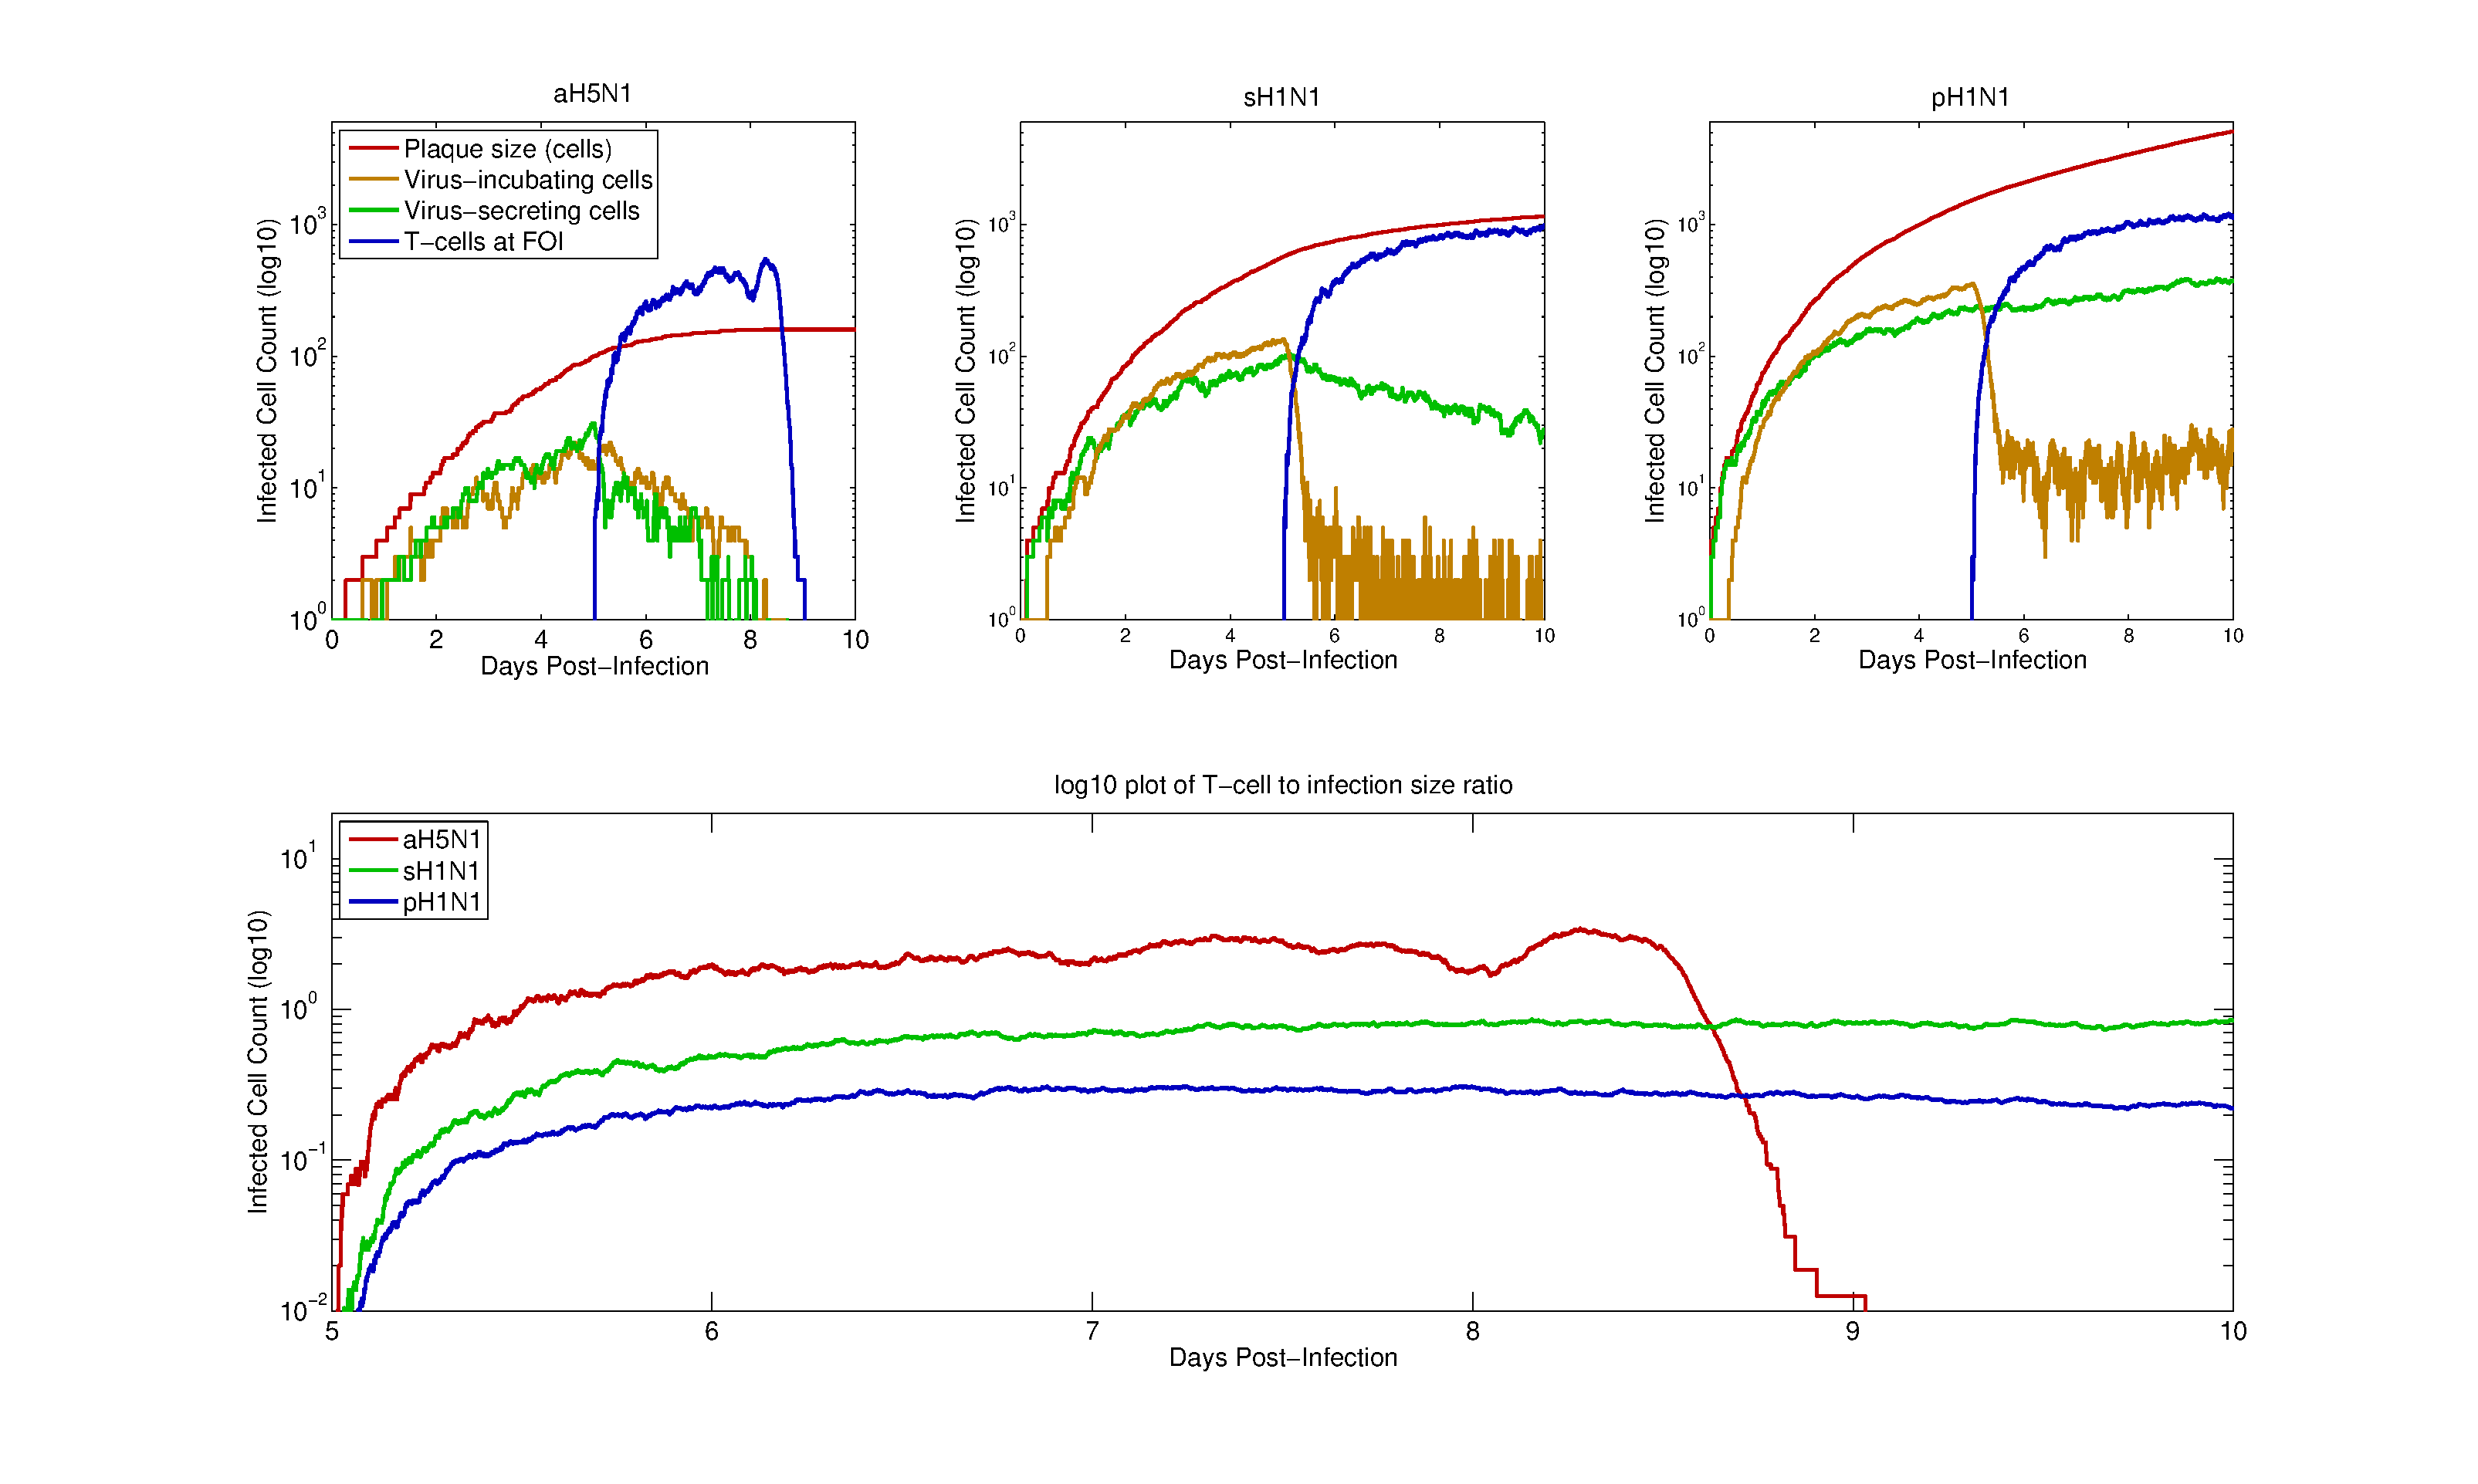
\includegraphics[width=\textwidth]{plaquesize}
 \end{center}
\caption{Comparison of total plaque size (green), number of virus incubating cells (blue), number of virus secreting cells (red), and T-cells (indigo) for the simulated infections of H5N1, sH1N1, and pH1N1.} 
 \label{fig:plaquesize}
\end{figure}


\section*{Discussion}


\subsection*{Chemokine Directed T-cell Search}

Hypercytokinemia is a characteristic of virulent influenza strains \cite{DeJong2006} but bloodstream levels of cytokines and chemokines may not reflect local concentrations and dynamics critical in guiding T cells to infected epithelial cells.  We elected to use our data on in vitro secretion of chemokines by human bronchial epithelial (NHBE) cells obtained from the same cultures of the three virus strains previously reported \cite{Mitchell2011}.  In this study the replication kinetics and productivity of the three virus strains were markedly different, but monolayer infection was initiated with a low MOI of 0.01 or 0.001, mimicking the initial infection naturally.  The levels of the chemokines CCL5 and CXCL10 in the basal media induced by the 3 strains were approximately equivalent at 24h post-infection.  When the productivity per cell was calculated, the avian H5N1 strain induced higher secretion of CCL5 (RANTES) than the seasonal or pandemic strains.  Greater CCL5 secretion by H5N1 strains has been noted in in vitro NHBE cultures when a relatively high MOI is used compared to seasonal strains \cite{Chan2005, Chan2010, Zeng2011} and pandemic strains \cite{Zeng2011}.  MOI and degree of differentiation of NHBE are critical determinants of cyto/chemokine secretion \cite{Chan2010}.  However, in spite of the attenuated type 1 interferon response induced by H5N1 strains \cite{Zeng2007}, the chemokine secretion is not attenuated.

Chemokines with a clear role directing T cell traffic include CXCL10 \cite{Dufour2002}, CCL5 \cite{Kawai1999} and CCL3 \cite{Kawai1999}.  The chemokine receptor CCR5, binding CCL5 and other chemokines, is crucial in the accelerated recruitment of CD8+ T cells to lung airways \cite{Kohlmeier2008}.  Other chemokines are likely to play a role in T cell traffic.  Although we did not detect significant levels of other chemokines in our cultures, the neutrophil- and T cell-attractant CXCL8/IL-8 is secreted into seasonal influenza-infected NHBE cultures \cite{Matsukura1996, Arndt2002}.  In the intact animal immigrant inflammatory cells particularly macrophages augment the multiple chemokine signals \cite{Julkunen2000}.  Finally, antigen-specific CD8+ T cell recognition of its target will induced lung injury mediated by TNFa and trigger addition alveolar epithelial cell chemokine secretion \cite{Zhao2000}.   Thus our model represents only a portion of the complete chemokine signal complex operating in the infected animal.

A key determinant in the efficiency of chemokine-directed T cell migration towards virus-secreting epithelial cells is the communication distance, defined by the threshold of sufficient chemokine signal to induce directed motion of the cell up the chemical gradient \cite{Thelen2008}.  The diameter of this cloud generated by a single cell is a function of production rate, decay rate, protein diffusion and the sensitivity threshold.  For the threshold of 10 pg/mL and maximal levels of concentration in tissue of 10,000 pg/mL, we calculated the effective communication distance as approximately 250 microns in our model.  This calculation matches the distance calculated for generic cytokines secreted by a suspended solitary cell \cite{Francis1997}.

\subsection*{General Immune Response Modeling}

The adaptive immune response to influenza in the mouse is a complex network of molecular and cellular elements, and incorporation of all of these into a comprehensive predictive model is not yet achieved.  Recent whole-animal models using a data-fitting approach and extensive databases have enhanced our global understanding of response metrics that are difficult or impossible to measure.  We have focused exclusively on the problem of the search of activated CTL for infected foci in the lung, and as in other models have made a number of assumptions.

Our focus on the T cell search necessitated the simplification or removal of selected features of the mammalian immune response, in order to permit tractable simulations.  Antigen presentation and peripheral lymphoid tissue amplification of the T cell clonal response is represented solely by the constant rate of emigration of activated T cells from regional lymph nodes.  Virus-specific strain replication rates are represented as constant rates, and virus clearance is also constant.  The contribution of IgM antibody clearing free virus is represented at a constant rate, and the class switch to higher affinity antibody mediated by CD4+ T cells is not represented.  All of these rates may in fact be time-variable rates as indicated by superior data-fitting models [Wu 2011].  Immigration and contributions of virus-nonspecific immune cells such as macrophages are not represented in our model.  Finally, the proliferation of activated T cells in lung tissue is not represented, but is thought to be crucial in the control of lung infection [Miao 2010].  Since known critical components were omitted or simplified, our model was not designed to demonstrate clearance of virus from the lung.  Rather our goal was to examine the features of the response that permitted T cells to sense and contact infected target cells.


\subsection*{ABM Advantages}

The use of an ABM has certain advantages over a spatially homogeneous ODE model.  An ODE model assumes that any virus particle is capable of infecting any healthy cell.  Figure \ref{fig:cycells} shows that this is clearly not the case.  In fact, most free virus exists on top of infected cells that are no longer candidates for viral binding and fusion.  ODE models account for this discrepancy by lowering rates of infection by a constant amount, but this assumes that the proportion of unsuitable virions will always be the same.  This is problematic as can been seen in Figure~\ref{fig:cycells} where the early infection has a higher proportion of virus overlapping healthy cells.

Our ABM renders the model in OpenGL (Fig.~\ref{fig:cycells}).  Seeing the model in action reveals spatial dynamics that are absent in ODEs and difficult or impossible to observe in \textit{in vitro} and \textit{in vivo} systems.  For example, observing the simulation reveals the spatial dynamics discussed in the Results.  We observed three key phenomena.  First, because T-cells find infected cells by climbing a gradient, we see T-cell clustering at local maxima of chemokine concentration, a posssible explanation for why T-cells do not increase in effectiveness as their numbers increase.  Second, T-cells bunching persists after all virus-secreting cells have been eliminated.  The local chemokine maxima takes time to diffuse and decay so that T-cells can climb the gradient to a new maximum.  Finally, we can see that infected cells are more disperse as infection size grows.  Because T-cells are clustered they cannot cover the increasing plaque effectively.  These spatial observations provide explanations for the pH1N1 resurgence that would be obscured without the visualization tools provided by the ABM.

% Do NOT remove this, even if you are not including acknowledgments
\section*{Acknowledgments}


\section*{References}
% The bibtex filename
\bibliography{references}

\section*{Figure Legends}
%\begin{figure}[!ht]
%\begin{center}
%%\includegraphics[width=4in]{figure_name.2.eps}
%\end{center}
%\caption{
%{\bf Bold the first sentence.}  Rest of figure 2  caption.  Caption 
%should be left justified, as specified by the options to the caption 
%package.
%}
%\label{Figure_label}
%\end{figure}


\section*{Tables}
%\begin{table}[!ht]
%\caption{
%\bf{Table title}}
%\begin{tabular}{|c|c|c|}
%table information
%\end{tabular}
%\begin{flushleft}Table caption
%\end{flushleft}
%\label{tab:label}
% \end{table}

\end{document}

